\documentclass[11pt]{amsart}
\usepackage[margin=1.1in]{geometry}
\usepackage{amssymb,amsmath,amsthm,booktabs,array,xcolor,url}
\usepackage{tikz}
\usepackage[hidelinks]{hyperref}
\newtheorem{theorem}{Theorem}
\newtheorem{lemma}[theorem]{Lemma}
\newtheorem{proposition}[theorem]{Proposition}
\theoremstyle{definition}
\newtheorem{definition}[theorem]{Definition}
\newtheorem{example}[theorem]{Example}
\theoremstyle{remark}
\newtheorem{remark}[theorem]{Remark}
\newcommand{\R}{R}
\newcommand{\lexle}{\preceq_{\mathrm{lex}}}

\title[The cycle Ramsey numbers $R(C_4,C_7,C_7)$ and $R(C_6,C_7,C_7)$]{The three-colour cycle Ramsey numbers\\ $R(C_4,C_7,C_7)$ and $R(C_6,C_7,C_7)$}
\author{Larsen Cundric}
\makeatletter\let\rl@origsetauthors\@setauthors
\def\@setauthors{\rl@origsetauthors\par\vspace{0.5em}{\centering\normalfont\small\itshape AI-generated manuscript produced using Grok Bot\\ Experiment initiated and guided by Larsen Cundric\par}}\makeatother
\date{Draft of \today}
\subjclass[2020]{05C55, 05D10, 68V15}
\keywords{Ramsey numbers, cycles, SAT solving, cube-and-conquer, proof certificates}

\begin{document}

\begin{abstract}
For graphs $G_1,G_2,G_3$, the Ramsey number $R(G_1,G_2,G_3)$ is the least $N$ such that every $3$-colouring of the edges of
$K_N$ contains a copy of $G_i$ in colour $i$ for some $i$. In the table of three-colour cycle Ramsey numbers
$R(C_m,C_n,C_k)$ with $m,n,k\le 7$ in Radziszowski's dynamic survey, the only entries without a value are
$R(C_m,C_7,C_7)$ for $m=3,4,5,6$. We show that $R(C_4,C_7,C_7)=15$ and $R(C_6,C_7,C_7)=21$.
The lower bounds come from explicit colourings. The upper bounds come from a SAT-based cube-and-conquer
computation in which forbidden-cycle clauses are generated lazily. Every part of it is certified: each clause the solver uses
is independently checked to be a genuine forbidden-cycle, colouring, or symmetry-breaking clause; every subproblem has an
unsatisfiability proof checked by the formally verified checker \texttt{cake\_lpr}; and the cube split is covered by a separate
checked certificate. An independent re-check of the upper bound for $R(C_4,C_7,C_7)$, with a different encoding,
symmetry-breaking scheme, lazy solver, cube split and proof checker (DRAT with \texttt{drat-trim}), is in progress; a
corresponding re-check for $R(C_6,C_7,C_7)$ will follow. We also give colourings showing $R(C_3,C_7,C_7)\ge 25$ and
$R(C_5,C_7,C_7)\ge 25$.
\end{abstract}

\maketitle

\section{Introduction}

\subsection*{The results in plain terms}
Colour every edge of a complete graph on $15$ vertices with one of three colours. Our first result says that, however this is
done, one always finds a cycle of length~$4$ in the first colour or a cycle of length~$7$ in the second or third colour, and that
$14$ vertices are not enough to force this. Our second result says the same for $21$ vertices with a $6$-cycle in the first colour
(with $20$ vertices not enough). For~$14$ and~$20$ vertices we exhibit colourings that avoid the forbidden cycles. For $15$
and~$21$ vertices we show by a certified computer search that no such colouring exists.

\subsection*{Definitions and statements}
All graphs are finite and simple, and $C_k$ is the cycle of length $k$. For graphs $G_1,\dots,G_r$ the Ramsey number
$R(G_1,\dots,G_r)$ is the least $N$ such that every colouring of $E(K_N)$ with colours $1,\dots,r$ has, for some $i$, a copy of
$G_i$ all of whose edges have colour $i$. A colouring of $K_{N-1}$ with no such copy is called \emph{good}; it shows $R>N-1$.
Below, the cycle lengths are assigned to colours $0,1,2$ in the order written: a colouring is good for
$(C_m,C_7,C_7)$ if colour~$0$ has no $C_m$ and colours $1$ and $2$ have no $C_7$.

\begin{theorem}\label{thm:main}
$R(C_4,C_7,C_7)=15$.
\end{theorem}

\begin{theorem}\label{thm:c6}
$R(C_6,C_7,C_7)=21$.
\end{theorem}

\begin{proposition}\label{prop:odd}
$R(C_3,C_7,C_7)\ge 25$ and $R(C_5,C_7,C_7)\ge 25$.
\end{proposition}

\subsection*{Background}
Radziszowski's dynamic survey~\cite{Rad} (revision~18, April 2026) collects all known values of three-colour cycle Ramsey numbers
in its Section~6.3.1 and Table~XII. Erd\H{o}s, Faudree, Rousseau and Schelp~\cite{EFRS1} determined $R(C_m,C_n,C_k)$ for
large~$m$ (formulas quoted in~\cite[6.3.1(a)]{Rad}). For three equal odd cycles, the conjecture attributed to Bondy and Erd\H{o}s
that $R(C_n,C_n,C_n)=4n-3$ for odd $n\ge5$ (see~\cite[6.3.1]{Rad}) was proved for large~$n$ by Kohayakawa, Simonovits and Skokan
(announced in~\cite{KoSS1}; see~\cite[6.3.1]{Rad} for the full proof), and $R(C_7,C_7,C_7)=25$ was proved without computer
support by Faudree, Schelten and Schiermeyer~\cite{FSS3}. Most of the small off-diagonal values in Table~XII of~\cite{Rad} were
obtained by computer, mainly by Sun, Yang, Wang, Li and Xu~\cite{SunYWLX} and Sun, Yang, Lin and Zheng~\cite{SunYLZ2}, and
independently by Tse~\cite{Tse3}. More recently, Lidick\'y and Pfender~\cite{LidP} used flag algebras, and Wesley~\cite{We3}
used SAT solvers to prove $R(C_3,C_6,C_6)=R(C_5,C_6,C_6)=15$.

In Table~XII of~\cite{Rad} (all $m\le n\le k\le 7$, plus $m=n=k=8$), exactly four entries are blank: $R(C_3,C_7,C_7)$,
$R(C_4,C_7,C_7)$, $R(C_5,C_7,C_7)$ and $R(C_6,C_7,C_7)$. According to the abstract of~\cite{SunYWLX}, that work treats
$R(C_{m_0},C_{m_1},C_{m_2})$ with $m_2\le m_1<m_0\le 7$, so the case where the two longer cycles have equal length~$7$ falls
outside it. We searched arXiv, Google Scholar, MathOverflow and Chinese-language sources (as of October~2026) and found no claimed
value for any of the four entries; we cannot rule out unindexed Chinese-language work.

\subsection*{How the upper bounds are proved}
The statement ``$K_n$ has a good colouring'' is a finite propositional formula, so the upper bounds amount to showing that certain
formulas are unsatisfiable. These formulas are large: the full CNF encoding for $K_{15}$ has about $4.6$ million clauses, and for
$K_{21}$ the $C_7$-clauses alone number about $8.4\times10^7$. We therefore (i) add forbidden-cycle clauses only when a solver
needs them, (ii) split the search into many small subproblems (\emph{cube-and-conquer}~\cite{HKWB}), and (iii) make every step
produce a certificate that is checked independently of the programs that produced it. The solvers themselves are not trusted.

\subsection*{Roadmap}
Section~\ref{sec:lower} gives the lower-bound colourings, with a worked example. Section~\ref{sec:method} describes the encoding,
symmetry breaking, lazy clause generation and cube-and-conquer, and Section~\ref{sec:cert} states exactly what is certified and
why that suffices (Theorem~\ref{thm:cert}). Section~\ref{sec:results} proves Theorems~\ref{thm:main} and~\ref{thm:c6} and reports the
status of the independent re-checks. Section~\ref{sec:repro} covers reproducibility and the use of AI tools. Implementation details are
in Appendix~\ref{app:impl}, validation on known values in Appendix~\ref{app:valid}, and run statistics in Appendix~\ref{app:stats}.

\section{Lower bounds}\label{sec:lower}

All lower-bound colourings in this paper are \emph{block constructions}. The vertex set is split into a few groups. One colour is
used inside the groups, and the other colours are used between groups in a bipartite pattern. The colour inside the groups avoids
long cycles because each group is small, and the colours between groups avoid odd cycles because they are bipartite.

\begin{example}[the colouring of $K_{14}$]\label{ex:k14}
Figure~\ref{fig:k14} shows the colouring behind Proposition~\ref{prop:lb4}. Fourteen vertices are split into two groups $A,B$ of
six and two extra vertices $s_1,s_2$. To be good for $(C_4,C_7,C_7)$, colour~$0$ must contain no $4$-cycle and colours~$1$ and~$2$
no $7$-cycle. Here colour~$0$ consists of two stars, which contain no cycles at all. A $7$-cycle in colour~$1$ would need seven
vertices in one connected piece of colour~$1$, but each piece is a $K_6$. Colour~$2$ only joins the two sides
$A\cup\{s_1\}$ and $B\cup\{s_2\}$, so every colour-$2$ cycle alternates sides and has even length. The main theorem says that adding a
fifteenth vertex makes such a colouring impossible.
\end{example}

\begin{figure}[ht]
\centering
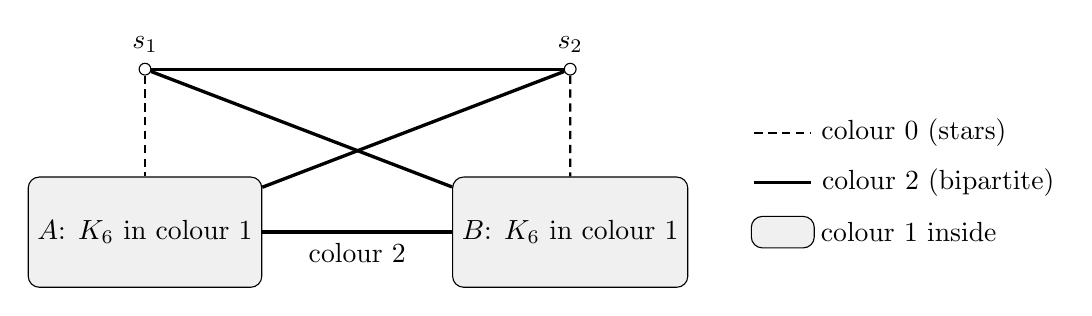
\begin{tikzpicture}[scale=0.9,
  grp/.style={draw,rounded corners,minimum width=2.2cm,minimum height=1.4cm,fill=gray!12},
  v/.style={circle,draw,fill=white,inner sep=1.5pt},
  c0/.style={densely dashed,thick},
  c2/.style={very thick}]
  \node[grp] (A) at (0,0) {$A$: $K_6$ in colour 1};
  \node[grp] (B) at (6,0) {$B$: $K_6$ in colour 1};
  \node[v,label=above:$s_1$] (s1) at (0,2.3) {};
  \node[v,label=above:$s_2$] (s2) at (6,2.3) {};
  \draw[c0] (s1) -- (A);
  \draw[c0] (s2) -- (B);
  \draw[c2] (A) -- node[below]{colour 2} (B);
  \draw[c2] (s1) -- (s2);
  \draw[c2] (s1) -- (B);
  \draw[c2] (s2) -- (A);
  \draw[c0] (8.6,1.4) -- (9.4,1.4) node[right]{colour 0 (stars)};
  \draw[c2] (8.6,0.7) -- (9.4,0.7) node[right]{colour 2 (bipartite)};
  \node[grp,minimum width=0.8cm,minimum height=0.4cm] at (9.0,0) {};
  \node[right] at (9.4,0) {colour 1 inside};
\end{tikzpicture}
\caption{A good colouring of $K_{14}$ for $(C_4,C_7,C_7)$. A line between a vertex or group and a group means all edges between
them have that colour.}\label{fig:k14}
\end{figure}

Each colouring below is also given as an explicit adjacency matrix in the accompanying artifact (Section~\ref{sec:repro}). Each
was checked with two independent programs: one using a depth-first search for monochromatic $k$-cycles, the other using the
\texttt{simple\_cycles} routine of NetworkX~3.7 with a length bound. The two checkers were cross-validated on 2730 random colourings
(0 disagreements), including brute-force enumeration on small instances.

\begin{proposition}\label{prop:lb4}
There is a good $3$-colouring of $K_{14}$ for $(C_4,C_7,C_7)$. Hence $R(C_4,C_7,C_7)\ge15$.
\end{proposition}
\begin{proof}
Let $V=A\cup B\cup\{s_1,s_2\}$ with $|A|=|B|=6$. Colour the edges inside $A$ and inside $B$ with colour~$1$; colour $s_1a$ ($a\in A$)
and $s_2b$ ($b\in B$) with colour~$0$; colour all other edges ($A$--$B$, $s_1$--$B$, $s_2$--$A$, $s_1s_2$) with colour~$2$.
Colour~$0$ is two disjoint stars $K_{1,6}$, which are acyclic. Colour~$1$ is two disjoint copies of $K_6$, so it has no cycle on $7$
vertices. Colour~$2$ is bipartite with parts $A\cup\{s_1\}$ and $B\cup\{s_2\}$, so it has no odd cycle.
\end{proof}

\begin{proposition}\label{prop:lb6}
There is a good $3$-colouring of $K_{20}$ for $(C_6,C_7,C_7)$. Hence $R(C_6,C_7,C_7)\ge21$.
\end{proposition}
\begin{proof}
Partition $V$ into $P_0,P_1,P_2,P_3$ of size $5$. Edges inside a part get colour $0$ (four disjoint $K_5$; no cycle of length
$6$). Edges between $P_0\cup P_1$ and $P_2\cup P_3$ get colour~$1$ (a $K_{10,10}$, bipartite). Edges between $P_0$ and $P_1$ and between $P_2$
and $P_3$ get colour $2$ (two disjoint copies of $K_{5,5}$, bipartite). Bipartite graphs contain no $C_7$.
\end{proof}

\begin{proof}[Proof of Proposition~\ref{prop:odd}]
Partition $V(K_{24})$ into $P_0,\dots,P_3$ of size $6$. Inside parts use colour~$1$ (four disjoint $K_6$, no $C_7$);
$P_0$--$P_1$ and $P_2$--$P_3$ use colour~$2$ (bipartite); $(P_0\cup P_1)$--$(P_2\cup P_3)$ uses colour $0$ (a $K_{12,12}$, which has
no odd cycle, in particular no $C_3$ and no $C_5$).
\end{proof}

\begin{remark}
These constructions agree with the values suggested by the neighbouring entries of Table~XII of~\cite{Rad}: for example
$R(C_3,C_5,C_7)=R(C_5,C_5,C_7)=R(C_7,C_7,C_7)=25$ and $R(C_6,C_6,C_7)=15$. An exhaustive search over circulant colourings found no
good circulant colouring of $K_{15}$ for $(C_4,C_7,C_7)$, of $K_{21}$ for $(C_6,C_7,C_7)$, or of $K_{25}$ for $(C_3,C_7,C_7)$ or
$(C_5,C_7,C_7)$.
\end{remark}

\section{Method}\label{sec:method}

Fix $n$ and lengths $L=(\ell_0,\ell_1,\ell_2)$ (here $\ell_0=m$, $\ell_1=\ell_2=7$). Write $E=\binom{[n]}{2}$, ordered
lexicographically. The computation was carried out in two independent \emph{legs}. Leg~A is the one on which
Theorems~\ref{thm:main} and~\ref{thm:c6} rest. Leg~B is an independent re-check with a different encoding, symmetry-breaking predicates, lazy solver, cube split, and proof
solver and checker (Appendix~\ref{app:impl}).

\subsection{Encoding}
In leg~A (Encoding~A) there are variables $x_{e,c}$ for $e\in E$, $c\in\{0,1,2\}$, meaning ``edge $e$ has colour $c$''. The clauses are:
\begin{itemize}
\item at-least-one: $x_{e,0}\vee x_{e,1}\vee x_{e,2}$ for every $e$;
\item at-most-one: $\neg x_{e,c}\vee\neg x_{e,c'}$ for $c<c'$;
\item forbidden cycles: for each colour $c$ and each $\ell_c$-cycle $Z$ of $K_n$, the clause $\bigvee_{e\in Z}\neg x_{e,c}$.
\end{itemize}
A satisfying assignment is exactly a good colouring. In a purely logical sense the at-most-one clauses are redundant (any model can
be reduced to one colour per edge), but they speed up solving considerably (Appendix~\ref{app:impl}). Leg~B uses a different
encoding, Encoding~B, with two variables per edge (Appendix~\ref{app:impl}).

\subsection{Symmetry breaking}\label{sec:sb}
The symmetric group $S_n$ acts on colourings by permuting vertices, and good colourings are mapped to good colourings, so it is enough
to look for one representative of each orbit. Fix a total order on the variables of the encoding, and for an assignment $\alpha$ write
$\alpha$ as a $0/1$ vector in that order. For a vertex permutation $\sigma$ let $\sigma\alpha$ be the assignment of the permuted
colouring, i.e.\ $(\sigma\alpha)(v_{\{i,j\},c})= \alpha(v_{\{\sigma^{-1}i,\sigma^{-1}j\},c})$.

\begin{lemma}[lex-leader, cf.~\cite{CGLR}]\label{lem:lexleader}
Let $T\subseteq S_n$ be any set of permutations and let $\Phi_T$ be a CNF over the original variables and fresh auxiliary variables such
that for every assignment $\alpha$ of the original variables with $\alpha\lexle\sigma\alpha$ for all $\sigma\in T$, some extension of
$\alpha$ to the auxiliary variables satisfies $\Phi_T$. If a good colouring of $K_n$ exists, then $F\wedge\Phi_T$ is satisfiable,
where $F$ is the full encoding (A or~B).
\end{lemma}
\begin{proof}
Let $\chi$ be good and let $\alpha^*$ be the lexicographically least assignment in the (finite) orbit $\{\sigma\alpha_\chi:\sigma\in
S_n\}$. Every element of the orbit encodes a good colouring and so satisfies $F$. For $\sigma\in T$, $\sigma\alpha^*$ also lies in the orbit, so
$\alpha^*\lexle\sigma\alpha^*$. By hypothesis $\alpha^*$ extends to a model of $\Phi_T$, and $F$ does not mention the auxiliary variables.
\end{proof}

We use $T=\{(i\ i{+}1):0\le i<n-1\}$ (adjacent transpositions). We encode $\alpha\lexle\sigma\alpha$ in the standard way: let
$X_1,\dots,X_p$ be the variables moved by $\sigma$ (in the variable order) and $Y_t$ the variable whose value $\sigma\alpha$ puts at
position $X_t$. With auxiliary variables $q_1,\dots,q_{p-1}$ (``equal so far''), the clauses are
\[
q_{t-1}\rightarrow(X_t\rightarrow Y_t),\qquad q_{t-1}\wedge(X_t\leftrightarrow Y_t)\rightarrow q_t\qquad(q_0:=\top).
\]
If $\alpha\lexle\sigma\alpha$, then setting $q_t$ true exactly when $X_s=Y_s$ for all $s\le t$ satisfies these clauses, so
Lemma~\ref{lem:lexleader} applies.

\subsection{Lazy cycle clauses}
For $\ell=7$ almost all clauses are cycle clauses: $K_{15}$ has $2{,}316{,}600$ seven-cycles, and $K_{21}$ has about
$4.19\times10^7$. We therefore start from a \emph{base formula}~$B$, which contains all colouring clauses, the symmetry-breaking
predicates, and the cycle clauses of length at most~$5$. Longer cycle clauses are added only when the solver's current partial
colouring closes a forbidden cycle (leg~A) or its candidate model contains one (leg~B); see Appendix~\ref{app:impl}. Every clause
added in this way is a forbidden-cycle clause of the full encoding, so it is implied by the encoding's semantics, and the procedure
is sound and complete. The added clauses are not trusted. They are written to a file and re-checked (Section~\ref{sec:cert}).

\subsection{Cube-and-conquer}
A \emph{cube} is a conjunction of literals, i.e.\ a partial colouring. We split the search space into cubes $Q_1,\dots,Q_s$ with the
look-ahead cuber \texttt{march\_cu}~\cite{HKWB}, and each cube is then solved separately. The split itself is not trusted: we only
use the resulting list of cubes, and its coverage is certified separately. For $K_{15}$, leg~A has $s=988$ cubes and leg~B has
$s=1022$; for $K_{21}$, leg~A has $s=1016$. A few cubes are far harder than the rest, so a cube that exceeds fixed time limits is
split again into subcubes $P\wedge D_1,\dots,P\wedge D_k$. The cubes therefore form a tree, whose leaves are solved
(Appendix~\ref{app:impl}).

\section{Certification}\label{sec:cert}

For each leg the certificate of ``no good colouring of $K_n$'' consists of the following.
\begin{enumerate}
\item[(C1)] \emph{Base legitimacy.} A separate checker reads $B$ clause by clause and accepts it only if every clause is a colouring
clause (at-least-one/at-most-one, or exclusion for~B), a genuine forbidden-cycle clause (its literals form a single cycle of the
forbidden length, in the right colour), or a symmetry-breaking clause regenerated from scratch.
\item[(C2)] \emph{Coverage.} The formula $\bigwedge_i\neg Q_i$ is unsatisfiable, so every assignment satisfies some cube.
\item[(C2$'$)] \emph{Split coverage.} For each split of a node $P$ into $P\wedge D_1,\dots,P\wedge D_k$, the formula
$P\wedge\bigwedge_j\neg D_j$ ($P$ as unit clauses) is unsatisfiable. As a fallback, $B\wedge P\wedge\bigwedge_j\neg D_j$ is unsatisfiable.
\item[(C3)] \emph{Cubes.} For each leaf $Q_i$ of the cube tree, let $E_i$ be the clauses added by the lazy solver while working under the assumptions $Q_i$.
The checker verifies that every clause of $E_i$ is a genuine forbidden-cycle clause. The formula $F_i=B\wedge E_i\wedge Q_i$ (with $Q_i$
as unit clauses) is then solved offline from scratch with proof logging, and the proof is checked.
\end{enumerate}

\begin{theorem}\label{thm:cert}
If (C1)--(C3) hold, then $K_n$ has no good colouring.
\end{theorem}
\begin{proof}
Suppose $\chi$ is good, and let $\alpha^*$ be the lex-least assignment in its orbit, extended to the auxiliary variables as in
Section~\ref{sec:sb}. By (C1) and Lemma~\ref{lem:lexleader}, $\alpha^*$ satisfies $B$. Each clause of $E_i$ forbids a monochromatic
$\ell_c$-cycle in colour~$c$, and $\alpha^*$ encodes a good colouring, so $\alpha^*$ satisfies every $E_i$. By (C2), $\alpha^*$
satisfies some top-level cube. By (C2$'$), whenever $\alpha^*$ satisfies a node $P$ that was split, it satisfies some child of $P$ (in the
fallback case, use that $\alpha^*$ satisfies $B$). Following the tree down, $\alpha^*$ satisfies some leaf $Q_j$, so it satisfies $F_j$. This contradicts the unsatisfiability of $F_j$ established in (C3).
\end{proof}

In leg~A each $F_i$ is solved by CaDiCaL~3.0.1~\cite{CaDiCaL2} with LRAT output, and the proof is checked by
\texttt{cake\_lpr}~\cite{cakelpr}, a checker that is verified in CakeML down to machine code. The coverage certificates are checked in
the same way. In leg~B the proofs are DRAT proofs from Kissat~4.0.4~\cite{Kissat24}, checked by \texttt{drat-trim}~\cite{DRATtrim}.
The two legs share neither a solver nor a proof checker. A separate audit script re-checks the bookkeeping and re-proves every
coverage formula with a second solver and checker (Appendix~\ref{app:impl}).

\section{Results}\label{sec:results}

\begin{proof}[Proof of Theorem~\ref{thm:main}]
The lower bound is Proposition~\ref{prop:lb4}. For the upper bound we applied Theorem~\ref{thm:cert} with $n=15$, using leg~A. The base
formula passes (C1). The coverage certificate (C2) for the $988$ cubes is verified by \texttt{cake\_lpr} and by \texttt{drat-trim}. All
$988$ cubes are UNSAT, with $E_i$ checked and LRAT proofs verified by \texttt{cake\_lpr} (C3). No cube needed re-splitting, and the
audit passes. Run statistics are in Appendix~\ref{app:stats}. The proof of the upper bound rests on leg~A.
\end{proof}

\begin{proof}[Proof of Theorem~\ref{thm:c6}]
The lower bound is Proposition~\ref{prop:lb6}. For the upper bound we applied Theorem~\ref{thm:cert} with $n=21$, using leg~A:
\begin{itemize}
\item The base formula passes the legitimacy check (C1), and the coverage certificate (C2) for the $1016$ top-level cubes is verified by
\texttt{cake\_lpr}.
\item $15$ top-level cubes exceeded the caps and were re-split, each into $64$ children ($960$ in total). Each of the $15$ split
coverage certificates (C2$'$) is verified by \texttt{cake\_lpr}.
\item The cube tree has $1961$ leaves ($1001$ unsplit top-level cubes and $960$ children). All $1961$ are UNSAT, with $E_i$ checked
and LRAT proofs verified by \texttt{cake\_lpr} (C3).
\item The audit passes: all $1016$ top-level cubes are certified, directly or through verified splits, and the top-level coverage and all
$15$ split coverages were re-proved with Kissat and \texttt{drat-trim}.
\end{itemize}
Run statistics are in Appendix~\ref{app:stats}.
\end{proof}

\begin{remark}[Independent re-checks, in progress]\label{rem:legB}
Leg~B for $n=15$ uses Encoding~B, its own symmetry-breaking predicates, its own lazy solver, and a different cube split
($1022$ top-level cubes), with Kissat DRAT proofs checked by \texttt{drat-trim}. Its coverage certificate has been verified both by
\texttt{drat-trim} and by \texttt{cake\_lpr}. This re-check is still running. As of 11~October~2026, $792$ of the $1022$ top-level
cubes have been certified, all of them UNSAT, and no good colouring has been found. An independent leg~B computation for $n=21$ has not
yet been run; it will start once the leg~B re-check for $n=15$ has finished. We will report both results, with their audits, in a
revised version.
\end{remark}

\begin{table}[ht]
\caption{The four previously open entries of Table~XII of~\cite{Rad}.}\label{tab:results}
\begin{tabular}{lccl}
\toprule
 & lower bound & upper bound & status \\
\midrule
$R(C_3,C_7,C_7)$ & $25$ (Prop.~\ref{prop:odd}) & -- & open \\
$R(C_4,C_7,C_7)$ & $15$ (Prop.~\ref{prop:lb4}) & $15$ (certified) & $=15$ \\
$R(C_5,C_7,C_7)$ & $25$ (Prop.~\ref{prop:odd}) & -- & open \\
$R(C_6,C_7,C_7)$ & $21$ (Prop.~\ref{prop:lb6}) & $21$ (certified) & $=21$ \\
\bottomrule
\end{tabular}
\end{table}

\begin{remark}
For $m\in\{3,5\}$ the corresponding computation on $K_{25}$ is beyond the methods used here. One possible route is a hybrid of the
Faudree--Schelten--Schiermeyer argument~\cite{FSS3} and SAT-checked local lemmas; we leave this open.
\end{remark}

\section{Reproducibility, data availability and use of AI tools}\label{sec:repro}

\subsection*{Data and code}
The artifact contains all generators, checkers, solver drivers, cube files, logs, per-cube status records with proof hashes, the
colourings, and a README with exact commands and SHA-256 checksums. Per-subproblem proof files were deleted after a successful check;
their sizes and SHA-256 hashes are kept. The artifact has not yet been deposited in a public archive; it is available from the author on
request. Tool versions and hardware are listed in Appendix~\ref{app:stats}.

\subsection*{Use of AI tools}
This is a personal project of the author, and the manuscript was produced using Grok Bot, an AI agent. The literature search, the
design and implementation of the encodings, checkers and solver drivers, the running of the computations, and the drafting of this
text, including the proofs, were done by the AI agent. The upper bounds do not rely on trusting the AI-written solvers: every
subproblem's unsatisfiability proof and every coverage certificate is checked by \texttt{cake\_lpr}, a formally verified proof checker,
and every clause added by a lazy solver is re-checked by a separate clause checker. What remains trusted is the symmetry-breaking
argument (Lemma~\ref{lem:lexleader}), the clause checkers, the assembly of the formulas $F_i$ (re-checked by the audit script), and the
coverage argument of Theorem~\ref{thm:cert}. The author initiated and guided this experiment but has not independently verified the
mathematics or the computations; the certificates are machine-checked as described above, but the paper has not been reviewed by a
human expert.

\appendix

\section{Implementation details}\label{app:impl}

\subsection*{Encoding A}
Cycles are enumerated once each by a depth-first search from the smallest vertex, with the second vertex smaller than the last. The
at-most-one clauses matter for speed: on $K_{12}$ for $(C_4,C_4,C_7)$, Kissat takes 143\,s with them and more than 20 minutes without them.

\subsection*{Encoding B (leg B)}
Variables $r_e, g_e$ for $e\in E$; colour $0$ is $r_e$, colour $1$ is $g_e$, colour $2$ is $\neg r_e\wedge\neg g_e$; clause
$\neg r_e\vee\neg g_e$. Forbidden cycles: $\bigvee_{e\in Z}\neg r_e$ for colour $0$, $\bigvee_{e\in Z}\neg g_e$ for colour $1$, and
$\bigvee_{e\in Z}(r_e\vee g_e)$ for colour $2$. Encoding~B was written separately from Encoding~A. Its generator enumerates cycles by
$k$-subsets and permutations, and its lazy solver uses its own depth-first search.

\subsection*{Symmetry-breaking predicates in the two legs}
Encodings A and~B use different variable sets and orders (A: $x_{e,0},x_{e,1},x_{e,2}$ per edge; B: $r_e,g_e$ per edge), so they lead
to different lexicographic orders and different symmetry-breaking predicates. As an additional check of the implementation, we tested
Encoding~B's predicates by brute force on $K_5$ and $K_6$: for random colourings, the lex-least member of the full $S_n$-orbit always
satisfied the predicates, while the lex-greatest member always violated them.

\subsection*{Lazy solvers}
In leg~A we use an external propagator for CaDiCaL~\cite{CaDiCaL2} through the IPASIR-UP interface~\cite{IPASIRUP}. It tracks the
partial colouring and, whenever the edges currently set to colour~$c$ close an $\ell_c$-cycle, adds that cycle's clause (which is then
falsified) as a conflict clause. It also checks every candidate model. In leg~B we use a counterexample-guided loop on top of
CaDiCaL~1.9.5 (through PySAT). We solve; if the model contains forbidden monochromatic cycles, we add up to $200$ of their clauses per
colour and solve again; otherwise the model is a good colouring.

\subsection*{Cubing and adaptive re-splitting}
Top-level cubes are produced by \texttt{march\_cu} at depth~$10$, run on $B$ together with the first $10^5$ cycle clauses from a short
lazy warm-up run. A few cubes are far harder than the rest; for example, two $K_{21}$ cubes took $32{,}392$\,s and $33{,}757$\,s of lazy
solving, while most take seconds. A cube (more generally, a node of the cube tree) is therefore split again when its lazy solve exceeds
$1200$\,s, or when its offline proof run or proof check exceeds $2400$\,s. To split node $P$ we run \texttt{march\_cu} (depth~$6$) on
$B$, together with up to $10^5$ of the cycle clauses the lazy solver had found under $P$ and the literals of $P$ as units. The result is
a list of subcubes $D_1,\dots,D_k$. The children of $P$ are $P\wedge D_j$, and the split is accepted only with a checked coverage
certificate (C2$'$).

\subsection*{Proof checking}
Before re-splitting was added, \texttt{drat-trim} needed up to $9.3$ hours on the proof of a single oversized cube in leg~B. With the caps
above, oversized cubes are split before their proofs grow that large. The coverage formula (C2) is checked in both ways in both legs.

\subsection*{Audit}
A separate audit script re-checks the bookkeeping: SHA-256 hashes of $B$ and the cube file are unchanged since the start, there is exactly
one certified record per cube, the literals in each record equal the cube in the file, and all verdicts are present. For every split, the
audit checks that each child's literals contain the parent's literals, and it re-proves the split's coverage formula itself (Kissat and
\texttt{drat-trim}) from the stored subcube files. It then checks that every top-level cube is certified, either directly or recursively
through its children. Proof files are deleted after a successful check; their sizes and SHA-256 hashes are kept in the logs.

\section{Validation on known values}\label{app:valid}
We ran the pipeline on known values and reproduced each of them:

\begin{center}
\begin{tabular}{ll>{\raggedright\arraybackslash}p{6.2cm}}
\toprule
value & result & checks \\
\midrule
$R(C_3,C_3,C_3)=17$ \cite{Rad} & $K_{16}$ SAT, $K_{17}$ UNSAT & \texttt{cake\_lpr}, \texttt{lrat-check}, \texttt{drat-trim} \\
$R(C_4,C_4,C_4)=11$ \cite{Rad} & $K_{10}$ SAT, $K_{11}$ UNSAT & \texttt{cake\_lpr}, \texttt{lrat-check}, \texttt{drat-trim} \\
$R(C_4,C_4,C_7)=12$ \cite{SunYLZ2,Tse3} & $K_{11}$ SAT, $K_{12}$ UNSAT & full CNF (both checkers); lazy C\&C legs A and B \\
$R(C_4,C_6,C_7)=13$ \cite{SunYWLX,Tse3} & $K_{12}$ SAT, $K_{13}$ UNSAT & full CNF (\texttt{cake\_lpr}, \texttt{lrat-check}, \texttt{drat-trim}); lazy C\&C leg A \\
\bottomrule
\end{tabular}
\end{center}
\noindent In addition, both lazy solvers found colourings of $K_{14}$ for $(C_4,C_7,C_7)$, and the C\&C driver correctly stopped
with a good colouring when run on $K_{12}$ for $(C_4,C_6,C_7)$. All such colourings passed both checkers. The clause checkers reject
deliberately corrupted clauses: a $C_4$-clause in a $C_7$-colour, a $C_7$-clause in the $C_4$-colour, a truncated cycle, and a
colouring clause offered as a cycle clause. Leg~B certified $R(C_4,C_4,C_7)\le 12$ ($K_{12}$, 121 cubes, all UNSAT, DRAT proofs verified by
\texttt{drat-trim}, coverage verified by \texttt{drat-trim} and \texttt{cake\_lpr}, audit passed). The cube-tree logic was tested on
$K_{12}$ by artificially capping solves at $2$\,s: this forced $13$ splits and $144$ leaves, and the audit passed. Deliberately deleting a
child from a split, or a leaf record, makes the audit fail.

\section{Run statistics, tools and hardware}\label{app:stats}

\subsection*{$K_{15}$, leg A (Theorem~\ref{thm:main})}
988 cubes, all certified. Total: 1672\,s lazy solving, 756\,s offline proof generation, and 338\,s proof checking; 16 minutes
wall-clock on 3 cores.

\subsection*{$K_{21}$, leg A (Theorem~\ref{thm:c6})}
For the $1961$ leaves, the computation took $152{,}289$\,s of lazy solving, $32{,}366$\,s of offline proof generation and $6{,}588$\,s of
proof checking. The $15$ runs that exceeded the caps used another $24{,}485$\,s, so the logged total is about $60$ core-hours. The run
took about $26$ hours wall-clock (8--9~October~2026, including restarts) with three worker processes.

\subsection*{$K_{15}$, leg B (in progress)}
As of 11~October~2026, $792$ of $1022$ top-level cubes are certified (all UNSAT). Leg~B is considerably slower than leg~A; it has been in
progress, with interruptions, since 8~October~2026.

\subsection*{Tools and hardware}
\begin{itemize}
\item CaDiCaL~3.0.1 (git \texttt{c607304}) and Kissat~4.0.4 (\texttt{8af8e56});
\item \texttt{cake\_lpr} (\texttt{a36874a}) and \texttt{drat-trim} (\texttt{2e3b2dc});
\item CnC/\texttt{march\_cu} (\texttt{705b60c});
\item PySAT~1.9.dev15 (with CaDiCaL~1.9.5), NetworkX~3.7 and Python~3.
\end{itemize}
All
computations ran on a single 8-core Intel Xeon virtual machine with 15\,GiB of RAM, which was shared with unrelated jobs. On this machine
the leg~A certificate for $K_{15}$ can be re-created in about 16 minutes on 3 cores, and the leg~A certificate for $K_{21}$ took about 60
core-hours.

\begin{thebibliography}{99}
\bibitem{CaDiCaL2} A.~Biere, T.~Faller, K.~Fazekas, M.~Fleury, N.~Froleyks and F.~Pollitt, CaDiCaL 2.0, in: \emph{Computer Aided
Verification (CAV 2024)}, LNCS 14681, Springer, 2024, 133--152, \url{https://doi.org/10.1007/978-3-031-65627-9_7}.
\bibitem{Kissat24} A.~Biere, T.~Faller, K.~Fazekas, M.~Fleury, N.~Froleyks and F.~Pollitt, CaDiCaL, Gimsatul, IsaSAT and Kissat entering
the SAT Competition 2024, in: \emph{Proc.\ SAT Competition 2024}, Dept.\ of Computer Science Report Series B, vol.\ B-2024-1,
University of Helsinki, 2024, 8--10.
\bibitem{CGLR} J.~Crawford, M.~Ginsberg, E.~Luks and A.~Roy, Symmetry-breaking predicates for search problems, in: \emph{Proc.\ KR'96},
Morgan Kaufmann, 1996, 148--159.
\bibitem{EFRS1} P.~Erd\H{o}s, R.\,J.~Faudree, C.\,C.~Rousseau and R.\,H.~Schelp, Generalized Ramsey theory for multiple colors,
\emph{J.\ Combin.\ Theory Ser.\ B} \textbf{20} (1976), 250--264, \url{https://doi.org/10.1016/0095-8956(76)90016-2}.
\bibitem{FSS3} R.\,J.~Faudree, A.~Schelten and I.~Schiermeyer, The Ramsey number $r(C_7,C_7,C_7)$, \emph{Discuss.\ Math.\ Graph
Theory} \textbf{23} (2003), 141--158, \url{https://doi.org/10.7151/dmgt.1191}.
\bibitem{IPASIRUP} K.~Fazekas, A.~Niemetz, M.~Preiner, M.~Kirchweger, S.~Szeider and A.~Biere, IPASIR-UP: user propagators for CDCL,
in: \emph{SAT 2023}, LIPIcs 271, 2023, 8:1--8:13, \url{https://doi.org/10.4230/LIPIcs.SAT.2023.8}.
\bibitem{HKWB} M.\,J.\,H.~Heule, O.~Kullmann, S.~Wieringa and A.~Biere, Cube and conquer: guiding CDCL SAT solvers by lookaheads,
in: \emph{HVC 2011}, LNCS 7261, Springer, 2012, 50--65, \url{https://doi.org/10.1007/978-3-642-34188-5_8}.
\bibitem{KoSS1} Y.~Kohayakawa, M.~Simonovits and J.~Skokan, The 3-colored Ramsey number of odd cycles, \emph{Electron.\ Notes
Discrete Math.} \textbf{19} (2005), 397--402, \url{https://doi.org/10.1016/j.endm.2005.05.053}.
\bibitem{LidP} B.~Lidick\'y and F.~Pfender, Semidefinite programming and Ramsey numbers, \emph{SIAM J.\ Discrete Math.} \textbf{35}(4)
(2021), 2328--2344, \url{https://doi.org/10.1137/18M1169473}.
\bibitem{Rad} S.\,P.~Radziszowski, Small Ramsey numbers, \emph{Electron.\ J.\ Combin.}, Dynamic Survey DS1, revision~18 (April 24,
2026), \url{https://doi.org/10.37236/21}.
\bibitem{SunYWLX} Sun Yongqi, Yang Yuansheng, Wang Wei, Li Bingxi and Xu Feng, Study of three color Ramsey numbers
$R(C_{m_1},C_{m_2},C_{m_3})$ (in Chinese), \emph{J.\ Dalian Univ.\ Technol.} \textbf{46} (2006), 428--433.
\bibitem{SunYLZ2} Sun Yongqi, Yang Yuansheng, Lin Xiaohui and Zheng Wenping, On the three color Ramsey numbers $R(C_m,C_4,C_4)$,
\emph{Ars Combin.} \textbf{84} (2007), 3--11.
\bibitem{cakelpr} Y.\,K.~Tan, M.\,J.\,H.~Heule and M.\,O.~Myreen, Verified propagation redundancy and compositional UNSAT checking in
CakeML, \emph{Int.\ J.\ Softw.\ Tools Technol.\ Transf.} \textbf{25} (2023), 167--184, \url{https://doi.org/10.1007/s10009-022-00690-y}.
\bibitem{Tse3} K.-K.~Tse, A note on some Ramsey numbers $R(C_p,C_q,C_r)$, \emph{J.\ Combin.\ Math.\ Combin.\ Comput.} \textbf{62}
(2007), 189--192.
\bibitem{We3} W.\,J.~Wesley, New bounds for some small multicolor Ramsey numbers, arXiv:2509.03784, 2025,
\url{https://doi.org/10.48550/arXiv.2509.03784}.
\bibitem{DRATtrim} N.~Wetzler, M.\,J.\,H.~Heule and W.\,A.~Hunt Jr., DRAT-trim: efficient checking and trimming using expressive
clausal proofs, in: \emph{SAT 2014}, LNCS 8561, Springer, 2014, 422--429, \url{https://doi.org/10.1007/978-3-319-09284-3_31}.
\end{thebibliography}

\end{document}
